\bibliographystyle{babplain-fl}

\chapter{Análisis de Union-Find}
\label{cha:analisis-de-union-find}

  Vimos que la estructura union-find,
  como discutida el capítulo~\ref{cha:algoritmo-de-kruskal},
  es central en varios algoritmos,
  corresponde evaluar su rendimiento.
  Las técnicas empleadas son instructivas,
  las expandiremos en clases sucesivas.

\section{Análisis de la versión simple}
\label{sec:union-find-analisys-simple}

  Veamos algunas propiedades cruciales de nuestra estructura inicial
  bajo las operaciones mencionadas:
  \begin{enumerate}[label = {\textbf{Propiedad \arabic*:}},
                    ref = \arabic*,
                    leftmargin = *,
                    itemindent = 4em]
  \item
    \label{prop:ufs-1}
    \emph{Para todo \(v\) que no es raíz,
          \(\mathrm{rank}[v]
               < \mathrm{rank}[\mathrm{parent}[v]]\).}

    \begin{proof}
      Un nodo de rango \(k\) se crea al unir dos árboles de rango \(k - 1\),
      una vez que un nodo deja de ser raíz su rango no se modifica más.
    \end{proof}
  \item
    \label{prop:ufs-2}
    \emph{Una raíz de rango \(k\) tiene al menos \(2^k\) nodos en su árbol.}

    \begin{proof}
      Una simple inducción.
      Esto se aplica a nodos internos
      (no raíz)
      también:
      un nodo de rango \(k\) tiene al menos \(2^k\) descendientes,
      ya que alguna vez fue raíz
      y una vez que deja de serlo su rango y sus descendientes no cambian más.
    \end{proof}
  \item
    \label{prop:ufs-3}
    \emph{Si hay un total de \(n\) nodos,
          hay a lo más \(n / 2^k\) nodos de rango \(k\).}

    \begin{proof}
      Considere su valor favorito \(k\),
      y cada vez que \(\mathrm{rank}\)
      de un nodo \(x\)
      cambia de \(k - 1\) a \(k\) marque todos sus descendientes.
      Cada nodo puede ser marcado a lo más una vez,
      ya que el rango de la raíz solo aumenta.
      Un nodo con rango \(k\)
      representa al menos a \(2^k\) nodos,
      habiendo un total de \(n\) nodos,
      hay a lo más \(n / 2^k\) nodos de rango \(k\).
    \end{proof}
    Esta observación indica,
    crucialmente,
    que el rango máximo es \(\log_2 n\),
    con lo que todos los árboles tienen altura a lo más \(\log_2 n\),
    y esta es una cota superior
    al tiempo de ejecución de \(\operatorname{find}\)
    y de \(\operatorname{union}\).
  \end{enumerate}

  Resulta que la cota de altura \(\log_2 n\) es ajustada,
  el árbol binomial \(B_k\)
  (construido uniendo dos árboles binomiales \(B_{k - 1}\),
   poniendo la raíz de uno como hijo de la raíz del otro,
   ver figura~\ref{fig:binomial-trees})
  tiene \(2^k\) nodos y altura \(k\).
  \begin{figure}[ht]
    \centering
    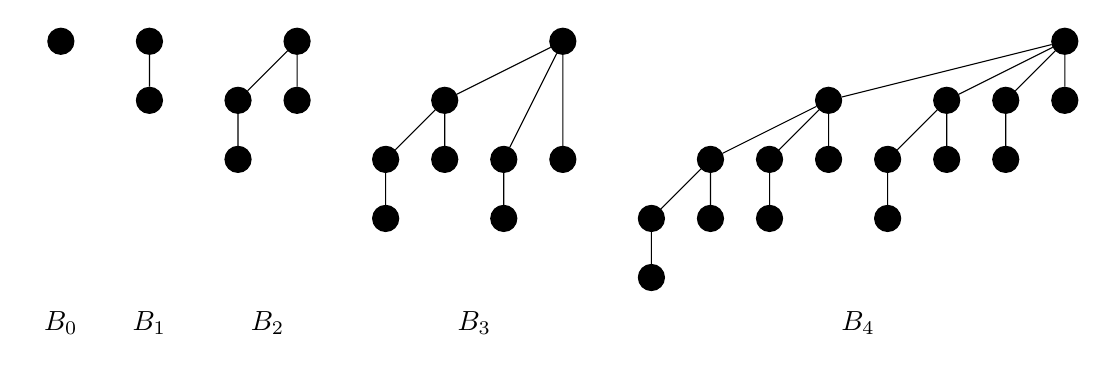
\begin{tikzpicture}[every node/.style = {shape = circle, fill, draw},
                        scale = 0.75]
      \node (a0) at (0, 4) {};
      \node [draw = none, fill = none, below] at (0, -0.2) {\(B_0\)};

      \node (b0) at (1.5, 3) {};
      \node (b1) at (1.5, 4) {};
      \draw (b0) -- (b1);
      \node [draw = none, fill = none, below] at (1.5, -0.2) {\(B_1\)};

      \node (c0) at (3.0, 2) {};
      \node (c1) at (3.0, 3) {};
      \node (c2) at (4.0, 3) {};
      \node (c3) at (4.0, 4) {};
      \draw (c0) -- (c1)
            (c1) -- (c3)
            (c2) -- (c3);
      \node [draw = none, fill = none, below] at (3.5, -0.2) {\(B_2\)};

      \node (d0) at (5.5, 1) {};
      \node (d1) at (5.5, 2) {};
      \node (d2) at (6.5, 2) {};
      \node (d3) at (6.5, 3) {};
      \node (d4) at (7.5, 1) {};
      \node (d5) at (7.5, 2) {};
      \node (d6) at (8.5, 2) {};
      \node (d7) at (8.5, 4) {};
      \draw (d0) -- (d1)
            (d1) -- (d3)
            (d2) -- (d3)
            (d4) -- (d5)
            (d6) -- (d7)
            (d3) -- (d7)
            (d5) -- (d7);
      \node [draw = none, fill = none, below] at (7, -0.2) {\(B_3\)};

      \node (e0)  at (10, 0) {};
      \node (e1)  at (10, 1) {};
      \node (e2)  at (11, 1) {};
      \node (e3)  at (11, 2) {};
      \node (e4)  at (12, 1) {};
      \node (e5)  at (12, 2) {};
      \node (e6)  at (13, 2) {};
      \node (e7)  at (13, 3) {};
      \node (e8)  at (14, 1) {};
      \node (e9)  at (14, 2) {};
      \node (e10) at (15, 2) {};
      \node (e11) at (15, 3) {};
      \node (e12) at (16, 2) {};
      \node (e13) at (16, 3) {};
      \node (e14) at (17, 3) {};
      \node (e15) at (17, 4) {};
      \draw (e0) -- (e1)
            (e1) -- (e3)
            (e2) -- (e3)
            (e4) -- (e5)
            (e6) -- (e7)
            (e3) -- (e7)
            (e5) -- (e7)
            (e8) -- (e9)
            (e9) -- (e11)
            (e10) -- (e11)
            (e12) -- (e13)
            (e13) -- (e15)
            (e14) -- (e15)
            (e11) -- (e15)
            (e7) -- (e15);
      \node [draw = none, fill = none, below] at (13.5, -0.2) {\(B_4\)};
    \end{tikzpicture}
    \caption{Árboles binomiales}
    \label{fig:binomial-trees}
\end{figure}

\section{Compresión de caminos}
\label{sec:union-find-path-compression}

  Una mejora se obtiene de la observación
  que luego de una búsqueda podemos acortar los caminos al representante
  a un solo paso
  para todos los nodos que encontramos en el camino,
  la figura~\ref{fig:union-find-path-compression}
  ilustra el efecto de buscar \num{20} y comprimir caminos.
  Si tenemos un puntero al nodo del que buscamos representante,
  recorremos la lista de padres hasta llegar a la raíz;
  en una segunda pasada sobre la lista ajustamos los punteros a padres
  para que apunten directamente a la raíz.
  Los árboles de las ilustraciones
  definitivamente no son resultado de nuestros algoritmos,
  simplemente sirven para mostrar el efecto de las operaciones.
  \begin{figure}[ht]
    \centering
    \begin{tikzpicture}
      \node at (0, 0) {\num{13}}
        child {node {\num{5}}}
        child {node {\num{6}}}
        child {node {\num{14}}
          child {node {\num{9}}
            child {node {\num{8}}}
            child {node {\num{16}}}
            child {node {\num{20}}
              child {node {\num{18}}}
              child {node {\num{19}}}}}};

        \node at (7, 0) {\num{13}}
          child {node {\num{5}}}
          child {node {\num{6}}}
          child {node {\num{9}}
            child {node {\num{8}}}
            child {node {\num{16}}}}
          child {node {\num{14}}}
          child {node {\num{20}}
            child {node {\num{18}}}
            child {node {\num{19}}}};
    \end{tikzpicture}
    \caption{Acortar caminos
             (\emph{\foreignlanguage{english}{path compression}})
             al buscar \num{20}.}
    \label{fig:union-find-path-compression}
  \end{figure}
  El algoritmo resultante~\ref{alg:union-find-find-2}
  es la versión modificada de \(\operatorname{find}\).
  \begin{algorithm}[ht]
    \DontPrintSemicolon\Indp

    \Function{\(\operatorname{find}(v)\)}{
      \(u \gets v\) \;
      \While{\(v \ne \mathrm{parent}[v]\)}{
        \(v \gets \mathrm{parent}[v]\) \;
      }
      \While{\(u \ne v\)}{
        \(p \gets \mathrm{parent}[u]\) \;
        \(\mathrm{parent}[u] \gets v\) \;
        \(u \gets p\) \;
      }
      \Return \(v\) \;
    }
    \caption{Algoritmo modificado para encontrar representante}
    \label{alg:union-find-find-2}
  \end{algorithm}
  La idea es pagar un costo extra en las operaciones \(\operatorname{find}\)
  en la esperanza de ahorrar en operaciones futuras.
  Una variante más simple es cambiar abuelos por padres
  en el recorrido de la lista,
  ahorrando un recorrido separado,
  ver el algoritmo~\ref{alg:union-find-find-3},
  que difiere del algoritmo original~\ref{alg:union-find-find}
  en una única línea.
  \begin{algorithm}[ht]
    \DontPrintSemicolon\Indp

    \Function{\(\operatorname{find}(v)\)}{
      \While{\(v \ne \mathrm{parent}[v]\)}{
        \(\mathrm{parent}[v]
            \gets \mathrm{parent}[\mathrm{parent}[v]]\) \;
        \(v \gets \mathrm{parent}[v]\) \;
      }
      \Return \(v\) \;
    }
    \caption{Algoritmo para encontrar representante con compresión de abuelos}
    \label{alg:union-find-find-3}
  \end{algorithm}
  La figura~\ref{fig:union-find-path-compression-grandparent}
  ilustra el efecto al buscar \num{19} usando esta variante.
  El algoritmo~\ref{alg:union-find-find-3}
  aprovecha que la raíz es su propio padre.
  \begin{figure}[ht]
    \centering
    \begin{tikzpicture}
      \node at (0, 0) {\num{13}}
        child {node {\num{5}}}
        child {node {\num{6}}}
        child {node {\num{14}}
          child {node {\num{9}}
            child {node {\num{8}}}
            child {node {\num{16}}}
            child {node {\num{20}}
              child {node {\num{18}}}
              child {node {\num{19}}}}}};

      \node at (7, 0) {\num{13}}
        child {node {\num{5}}}
        child {node {\num{6}}}
        child {node {\num{9}}
          child {node {\num{8}}}
          child {node {\num{16}}}}
        child {node {\num{14}}
          child {node {\num{20}}
            child {node {\num{18}}}
            child {node {\num{19}}}}};
    \end{tikzpicture}
    \caption{Acortar caminos
             (\emph{\foreignlanguage{english}{path compression}})
             con abuelos desde \num{20}.}
    \label{fig:union-find-path-compression-grandparent}
  \end{figure}

\section{Análisis de compresión de caminos}
\label{sec:union-find-analysis-path-compression}

  Como estamos pagando un costo extra en ciertas operaciones
  en la esperanza de que produzca ahorros futuros,
  debemos analizar secuencias de operaciones,
  no operaciones individuales.

  Para \(g \colon \mathbb{R} \to \mathbb{R}\)
  tal que para \(x > 1\) siempre es \(g(x) < x\) definimos:
  \begin{equation}
    \label{eq:def-g*}
    g^*(x)
      = \begin{cases}
          0		& x \le 1 \\
          1 + g^*(g(x))	& x >	1
        \end{cases}
  \end{equation}
  En el fondo, \(g^*(x)\) es el número de veces
  que hay que aplicar \(g\) a \(x\)
  hasta obtener un valor \num{1} o menor.
  De acá definimos \(\log_2^* x\),
  donde el logaritmo es en base \num{2}
  (¡somos computines!).
  Es claro que \(\log_2^* n\) crece extremadamente lento:
  \begin{equation*}
    \log_2^* n
      = \begin{cases}
           0 & \phantom{1 < {}}
                        n \le 1	  \\
           1 & 1      < n \le 2	  \\
           2 & 2      < n \le 2^2 \\
           3 & 2^2    < n \le 2^4 \\
           4 & 2^4    < n \le 2^{16} \\
           5 & 2^{16} < n \le 2^{65\,536}
        \end{cases}
  \end{equation*}

  El análisis clásico de esta estructura
  (Hopcroft y Ullman~\cite{hopcroft73:_set_merging_algorithm},
   Tarjan~\cite{tarjan75:_union-find_analysis})
  es complejo.
  Acá seguimos la idea de Seidel y Sharir~%
    \cite{seidel05:_top_down_analysis_path_compr},
  que da un análisis sencillo
  (todo depende del cristal con que se mira\ldots).
  Primeramente,
  las tres propiedades enunciadas antes se siguen cumpliendo
  aún si se comprimen caminos.
  Basan su análisis en dos nuevas operaciones,
  \(\operatorname{compress}(u, v)\)
  que comprime un camino cualquiera en el bosque
  (no necesariamente llegando a una raíz)
  entre nodos \(u\) y \(v\),
  donde \(v\) es un ancestro de \(u\),
  y la operación \(\operatorname{shatter}(u, v)\),
  que hace una raíz de todo nodo en el camino.
  \begin{algorithm}[ht]
    \DontPrintSemicolon\Indp

    \Procedure{\(\operatorname{compress}(u, v)\)}{
      \emph{\(v\) must be ancestor of \(u\)} \;
      \If{\(u \ne v\)}{
        \(\operatorname{compress}(\mathrm{parent}[u], v)\) \;
        \(\mathrm{parent}[u] \gets \mathrm{parent}[v]\) \;
      }
    }
    \caption{Operación \(\operatorname{compress}\)}
    \label{alg:uf-compress}
  \end{algorithm}
  \begin{algorithm}[ht]
    \DontPrintSemicolon\Indp

    \Procedure{\(\operatorname{shatter}(u, v)\)}{
      \emph{\(v\) must be ancestor of \(u\)} \;
      \If{\(\mathrm{parent}[u] \ne v\)}{
        \(\operatorname{shatter}(\mathrm{parent}[u], v)\) \;
       \(\mathrm{parent}[u] \gets u\) \;
      }
    }
    \caption{Operación \(\operatorname{shatter}\)}
    \label{alg:uf-shatter}
  \end{algorithm}
  Cabe hacer notar que estas operaciones no son para uso en el programa,
  sirven para reordenar las acciones simplificando las demostraciones.
  En particular,
  si \(\operatorname{union}\) no reorganiza los árboles,
  solo manipula las raíces,
  una secuencia cualquiera
  de \(\operatorname{union}\) y \(\operatorname{find}\)
  puede efectuarse haciendo las \(\operatorname{union}\),
  seguidas por \(\operatorname{compress}\)
  sin cambiar el número de manipulaciones de punteros.
  El costo de \(\operatorname{union}\) es constante
  (\(O(1)\)),
  \(\operatorname{find}\) es básicamente \(\operatorname{compress}\),
  que es \(O(1)\)
  más un término proporcional al número de punteros manipulados.
  Fijaremos entonces el número de punteros manipulados
  como medida de costo.
  Sea \(T(m, n, r)\) el número de asignaciones de punteros en el peor caso
  en cualquier secuencia de \(m\) operaciones \(\operatorname{compress}\)
  sobre un bosque de a lo más \(n\) nodos,
  con \(\mathrm{rank}\) a lo más \(r\).

  La siguiente cota trivial sirve de base a nuestro argumento.
  \begin{lemma}
    \label{lem:T-trivial}
    \(T(m, n, r) \le n r\)
  \end{lemma}
  \begin{proof}
    Cada nodo puede cambiar padre a lo más \(r\) veces,
    ya que \(\mathrm{rank}\) siempre aumenta.
  \end{proof}
  Sea \(\mathscr{F}\) un bosque de \(n\) nodos
  con \(\mathrm{rank}\) máximo \(r\)
  y una secuencia \(C\) de \(m\) operaciones \(\operatorname{compress}\)
  sobre \(\mathscr{F}\),
  y sea \(T(\mathscr{F}, C)\)
  el número total de asignaciones de punteros ejecutados por esta secuencia.
  Divida el bosque en dos subbosques,
  un bosque \textquote{bajo} \(\mathscr{F}_-\)
  con los nodos de \(\mathrm{rank}[v] \le s\)
  y el bosque \textquote{alto} \(\mathscr{F}_+\)
  con los nodos de \(\mathrm{rank}[v] > s\).
  Como \(\mathrm{rank}\) aumenta al seguir punteros a padres,
  el padre de un nodo alto es otro nodo alto.
  Sean \(n_-\) y \(n_+\) el número de nodos bajos y altos,
  respectivamente.
  Ver la figura~\ref{fig:union-find-subforests}
  que muestra un bosque
  (un único árbol en el ejemplo)
  dividido en subbosques.
  \begin{figure}[ht]
    \centering
    \begin{tikzpicture}[scale = 1.75]
      \draw [fill = lightgray] (0, 0) -- (-1.154, -2) -- (1.154, -2) -- cycle;
      \node at (0, -1) {\(\mathscr{F}\)};

      \draw [dashed] (-2, -1) -- (2, -1);
      \node at (0.7, -1) [above right]
        {\scriptsize\(\mathrm{rank} \ge s\)};
      \node at (0.7, -1) [below right]
        {\scriptsize\(\mathrm{rank} < s\)};

      \draw [fill = lightgray]
         (4, 0) -- (4 - 0.577, -1) -- (4 + 0.577, -1) -- cycle;
      \node at (4, -0.577) {\(\mathscr{F}_+\)};

      \draw [draw = none, fill = lightgray, pattern = dots]
            (4 + 0 * 0.144 - 0.577, -1) -- (4 + 0 * 0.144 - 1.154, -2) --
            (4 + 8 * 0.144, -2) -- (4 + 8 * 0.144 - 0.577, -1) --
            cycle;

      \draw (4 + 0 * 0.144 - 0.577, -1) -- (4 + 0 * 0.144 - 1.154, -2)
            (4 + 0 * 0.144 - 0.577, -1) -- (4 + 0 * 0.144, -2);
      \draw (4 + 2 * 0.144 - 0.577, -1) -- (4 + 2 * 0.144 - 1.154, -2)
            (4 + 2 * 0.144 - 0.577, -1) -- (4 + 2 * 0.144, -2);
      \draw (4 + 4 * 0.144 - 0.577, -1) -- (4 + 4 * 0.144 - 1.154, -2)
            (4 + 4 * 0.144 - 0.577, -1) -- (4 + 4 * 0.144, -2);
      \draw (4 + 6 * 0.144 - 0.577, -1) -- (4 + 6 * 0.144 - 1.154, -2)
            (4 + 6 * 0.144 - 0.577, -1) -- (4 + 6 * 0.144, -2);
      \draw (4 + 8 * 0.144 - 0.577, -1) -- (4 + 8 * 0.144 - 1.154, -2)
            (4 + 8 * 0.144 - 0.577, -1) -- (4 + 8 * 0.144, -2);

      \node at (4, -1.5) {\(\mathscr{F}_-\)};
    \end{tikzpicture}
    \caption{Dividiendo el bosque según \(\mathrm{rank}\)}
    \label{fig:union-find-subforests}
  \end{figure}

  Cualquier secuencia de operaciones \(\operatorname{compress}\)
  sobre \(\mathscr{F}\)
  puede descomponerse
  en una secuencia de operaciones \(\operatorname{compress}\)
  sobre \(\mathscr{F}_+\)
  y una secuencia de operaciones \(\operatorname{compress}\)
  y \(\operatorname{shatter}\) sobre \(\mathscr{F}_-\)
  con el mismo costo.
  La modificación es prohibir a un nodo bajo tener un padre alto,
  haciendo que los nodos bajos se hagan raíces
  y dejando a los nodos altos de hijos de la raíz original,
  como muestra la figura~\ref{fig:union-find-compress-+-}
  para un camino simple a la raíz que cruza de nodos bajos a altos..
  \begin{figure}[ht]
    \centering
    \begin{tikzpicture}
      \node [draw, shape = circle]    at (0, 0)			 (0) {}
          node [draw, shape = circle] at (-0.2 *  1, -0.5 *  1)	 (1) {}
          node [draw, shape = circle] at (-0.2 *  2, -0.5 *  2)	 (2) {}
          node [draw, shape = circle] at (-0.2 *  3, -0.5 *  3)	 (3) {}
          node [draw, shape = circle] at (-0.2 *  4, -0.5 *  4)	 (4) {}
          node [draw, shape = circle] at (-0.2 *  5, -0.5 *  5)	 (5) {}
          node [draw, shape = circle] at (-0.2 *  6, -0.5 *  6)	 (6) {}
          node [draw, shape = circle] at (-0.2 *  7, -0.5 *  7)	 (7) {}
          node [draw, shape = circle] at (-0.2 *  8, -0.5 *  8)	 (8) {}
          node [draw, shape = circle] at (-0.2 *  9, -0.5 *  9)	 (9) {}
          node [draw, shape = circle] at (-0.2 * 10, -0.5 * 10) (10) {};

      \draw[gray] (-0.2 * 5.5 - 0.5, -0.5 * 5.5)
                    -- (0.2 * 5.5 + 0.5, -0.5 * 5.5);

      \path[-latex'] (10) edge node {} (9)
                 (9) edge node {} (8)
                 (8) edge node {} (7)
                 (7) edge node {} (6)
                 (6) edge node {} (5)
                 (5) edge node {} (4)
                 (4) edge node {} (3)
                 (3) edge node {} (2)
                 (2) edge node {} (1)
                 (1) edge node {} (0)
                 (0) edge [loop above] node {} (0);


      \node [draw, shape = circle]    at (5, 0)		      (0) {}
          node [draw, shape = circle] at (5 - 0.4 * 2, -0.7)  (1) {}
          node [draw, shape = circle] at (5 - 0.4 * 1, -0.7)  (2) {}
          node [draw, shape = circle] at (5 + 0.4 * 0, -0.7)  (3) {}
          node [draw, shape = circle] at (5 + 0.4 * 1, -0.7)  (4) {}
          node [draw, shape = circle] at (5 + 0.4 * 2, -0.7)  (5) {};

      \path[-latex'] (0) edge [loop above] node {} (0)
                (1) edge	      node {} (0)
                (2) edge	      node {} (0)
                (3) edge	      node {} (0)
                (4) edge	      node {} (0)
                (5) edge	      node {} (0);

      \draw[gray] (5 + -0.2 * 5.5 - 0.5, -0.5 * 5.5)
                    -- (5 + 0.2 * 5.5 + 0.5, -0.5 * 5.5);

      \node [draw, shape = circle]    at (5 - 0.4 * 2, -0.5 * 6)  (a) {}
          node [draw, shape = circle] at (5 - 0.4 * 1, -0.5 * 6)  (b) {}
          node [draw, shape = circle] at (5 + 0.4 * 0, -0.5 * 6)  (c) {}
          node [draw, shape = circle] at (5 + 0.4 * 1, -0.5 * 6)  (d) {}
          node [draw, shape = circle] at (5 + 0.4 * 2, -0.5 * 6)  (e) {};

      \path[-latex'] (a) edge [loop above] node {} (a)
                (b) edge [loop above] node {} (b)
                (c) edge [loop above] node {} (c)
                (d) edge [loop above] node {} (d)
                (e) edge [loop above] node {} (e);
    \end{tikzpicture}
    \caption{División de una operación \(\operatorname{compress}\)}
    \label{fig:union-find-compress-+-}
  \end{figure}
  El punto de hacer esto es descomponer la secuencia en secuencias menores.
  Al dividir el bosque en nodos \textquote{altos} y \textquote{bajos},
  queda un bosque alto muy pequeño
  (son pocos los nodos con \(\mathrm{rank}\) alto),
  con lo que bastarán cotas bastante burdas
  para el costo de operaciones en él.
  El resultado es una recurrencia
  que acota el costo de la secuencia de operaciones.
  \begin{algorithm}[ht]
    \DontPrintSemicolon\Indp

    \Procedure{\(\operatorname{compress-rank}(u, v)\)}{
      \uIf{\(\mathrm{rank}[u] > s\)}{
        \(\operatorname{compress}(u, v)\) \;
      }
      \uElseIf{\(\mathrm{rank}[v] \le s\)}{
        \(\operatorname{compress}(u, v)\) \;
      }
      \Else{
        \(z \gets u\) \;
        \While{
          \(\mathrm{rank}[\mathrm{parent}[z]]
              \le s\)}{
          \(z \gets \mathrm{parent}[z]\) \;
        }
        \(\operatorname{compress}(\mathrm{parent}[z], v)\) \;
        \(\operatorname{shatter}(u, z)\) \;
        \(\mathrm{parent}[z] \gets z\) \;
      }
    }
    \caption{Operación equivalente}
    \label{alg:uf-compress-shatter}
  \end{algorithm}

  La operación \(\operatorname{compress}\) adaptada a bosques divididos
  considera el caso en que el camino \(u\) a \(v\)
  es enteramente \textquote{alto}
  (caso \(\mathrm{rank}[u] > s\)),
  enteramente \textquote{bajo}
  (cuando \(\mathrm{rank}[v] \le s\)),
  o cruza el rango y hay que subdividir la operación.

  La última asignación del algoritmo~\ref{alg:uf-compress-shatter}
  parece superflua,
  pero es necesaria en el análisis para simular una operación
  \(\mathrm{parent}[z] \leftarrow w\),
  con \(z\) un nodo bajo,
  \(w\) un nodo alto y el padre de \(z\) era un nodo alto también.
  Estas asignaciones \textquote{redundantes} se ejecutan inmediatamente después
  de una operación \(\operatorname{compress}\) en el bosque superior,
  por lo que hay a lo más \(m_+\) de estas operaciones.

  Durante la secuencia de operaciones \(C\) cada nodo es tocado
  por a lo más una operación \(\operatorname{shatter}\),
  por lo que el número total de operaciones con punteros en ellas
  es a lo más \(n\).

  Al dividir el bosque hemos dividido
  la secuencia de operaciones \(\operatorname{compress}\)
  en subsecuencias \(C_-\) y \(C_+\)
  de operaciones \(\operatorname{compress}\),
  de largos respectivos \(m_-\) y \(m_+\)
  (es \(m = m_+ + m_-\)),
  además de operaciones \(\operatorname{shatter}\).
  En vista de las consideraciones anteriores se cumple la desigualdad:
  \begin{equation}
    \label{eq:desigualdad-T}
    T(\mathscr{F}, C)
      \le T(\mathscr{F}_-, C_-) + T(\mathscr{F}_+, C_+) + m_+ + n
  \end{equation}
  Como hay a lo más \(n / 2^i\) nodos de rango \(i\),
  tenemos que:
  \begin{equation*}
    n_+
      \le \sum_{i > s} \frac{n}{2^i}
      = \frac{n}{2^s}
  \end{equation*}
  Con esto la cota del lema~\ref{lem:T-trivial}
  implica:
  \begin{equation*}
    T(\mathscr{F}_+, C_+)
      \le \frac{r n}{2^s}
  \end{equation*}
  Fijemos \(s = \lfloor \log_2 r \rfloor\),
  de manera que \(T(\mathscr{F}_+, C_+) \le n\).
  El bosque \(\mathscr{F}_-\)
  tiene \(\mathrm{rank}\) máximo \(s = \lfloor \log_2 r \rfloor\),
  además es claro que \(\lvert C_- \rvert \le \lvert C \rvert = m\).
  Podemos simplificar nuestra recurrencia a:
  \begin{equation*}
    T(\mathscr{F}, C)
      \le T(\mathscr{F}_-, C_-) + m_+ + 2 n
  \end{equation*}
  lo que con las observaciones previas es lo mismo que:
  \begin{equation*}
    T(\mathscr{F}, C) - m
      \le T(\mathscr{F}_-, C_-) - m_- + 2 n
  \end{equation*}
  Como esto vale en \emph{cualquier} bosque \(\mathscr{F}\)
  y para toda secuencia \(C\),
  y como \(T(m, n, r)\) es creciente con sus dos primeros argumentos,
  hemos demostrado que
  para \(T'(m, n, r) = T(m, n, r) - m\):
  \begin{align*}
    T'(m, n, r)
      &\le T'(m_-, n, \lfloor \log_2 r \rfloor) + 2 n \\
      &\le T'(m, n, \lfloor \log_2 r \rfloor) + 2 n
  \end{align*}
  Como condición inicial,
  para \(r = 1\) todos los nodos son raíces o hijos de una raíz,
  no hay manipulación de \(\mathrm{parent}\),
  y \(T'(m, n, 1) \le 0\).
  La solución a esta recurrencia es:
  \begin{equation*}
    T'(m, n, r)
      \le 2 n \log_2^* r
  \end{equation*}

  Hemos demostrado:
  \begin{theorem}
    \label{theo:T-log*}
    \(T(m, n, r)
      \le m + 2 n \log_2^* r\)
  \end{theorem}

  El teorema~\ref{theo:T-log*} puede mejorarse.
  En la demostración usamos la cota del lema~\ref{lem:T-trivial},
  que nuestro teorema~\ref{theo:T-log*} mejora,
  y puede usarse recursivamente,
  aumentando cada vez algo la dependencia de \(m\)
  mientras disminuye la de \(r\).
  Erickson~%
    \cite[clase~17]{erickson19:_algorithms}
  completa el desarrollo.
  Se concluye lo siguiente:
  La función de Ackermann~%
    \cite{ackermann28:_zum_hilbert_aufbau_zahlen}
  (aunque usamos la forma de dos argumentos definida por Péter~%
     \cite{peter34:_konstruktion_nichtrekursiver_funktionen}
   y Robinson~%
     \cite{robinson48:_recursion_double_recursion})
  se define como:
  \begin{equation*}
    \label{eq:Ackermann}
    A(m, n)
      = \begin{cases}
          n + 1			 & m = 0 \\
          A(m - 1, 1)		 & m > 0 \wedge n = 0 \\
          A(m - 1, A(m, n - 1))	 & m > 0 \wedge n > 0
        \end{cases}
  \end{equation*}
  Para algunos ejemplos,
  vemos que:
  \begin{align*}
    A(0, n)
      &= n + 1 \\
    A(1, n)
      &= A(0, A(1, n - 1)) \\
      &= A(1, n - 1) + 1 \\
      &\vdots \\
      &= A(1, 0) + n \\
      &= A(0, 1) + n \\
      &= n + 2 \\
      &= 2 + (n + 3) - 3 \\
    A(2, n)
      &= A(1, A(2, n - 1)) \\
      &= A(1, A(1, A(2, n - 2))) \\
      &\vdots \\
      &= A(1, A(1, A(1, \dotsc, A(1, A(2, 0)))) \\
      &= A(1, A(1, A(1, \dotsc, A(1, 3)) \\
      &\vdots \\
      &= 2 n + 3 \\
      &= 2 (n + 3) - 3 \\
    A(3, n)
      &= A(2, A(3, n - 1)) \\
      &\vdots \\
      &= A(2, A(2, A(2, \dotsc, A(2, A(2, 0))) \\
      &= A(2, A(2, A(2, \dotsc, A(2, 3))) \\
      &\vdots \\
      &= 2^{n + 3} - 3
  \end{align*}
  Esencialmente,
  cada aumento de \(m\) significa
  \textquote{aplique la función anterior \(n + 3\) veces},
  \(A(1, n)\) es \textquote{\(n + 3\) veces sumar \num{1}},
  \(A(2, n)\) es \textquote{\(n + 3\) veces sumar \num{2}},
  \(A(3, n)\) es \textquote{\(n + 3\) veces multiplicar por \num{2}},
  \(A(4, n)\) es \textquote{\(n + 3\) veces elevar a la potencia \num{2}},
  lo que da:
  \begin{equation*}
    A(4, n)
      = \begin{matrix}
          \underbrace{{2^2}^{{\cdot}^{{\cdot}^{{\cdot}^2}}}}_{n + 3} - 3
        \end{matrix}
  \end{equation*}
  O sea,
  por ejemplo:
  \begin{equation*}
    A(4, 3)
      = 2^{2^{65536}} - 3
  \end{equation*}
  Se ve que esta función crece extremadamente rápido.

  Se definen dos funciones inversas,
  que crecen extremadamente lento:
  \begin{align}
    \alpha(n)
      &= A^{-1}(n, n)
            \label{eq:alpha-1} \\
    \alpha(m, n)
      &= \min \{ i \ge 1 \colon A(i, \lfloor m / n \rfloor) \ge \log_2 n \}
            \label{eq:alpha-2}
  \end{align}
  De los valores anteriores para \(A(m, n)\)
  vemos que para todos los valores imaginables de \(m\) y \(n\)
  es \(\alpha(m, n) \le 5\).
  Claro que en estricto rigor no está acotada por una constante.

  En estos términos,
  Tarjan~%
    \cite{tarjan75:_union-find_analysis}
  demuestra que
  toda secuencia intercalada
  de \(m \ge n\) operaciones \(\operatorname{find}\)
  y \(n - 1\) operaciones \(\operatorname{union}\)
  toma \(O(m \alpha(m, n))\) tiempo.

  Volvamos al algoritmo de Kruskal,
  llamemos simplemente \(V\) y \(E\) al número de vértices y arcos,
  respectivamente.
  Se hacen a lo más \(2 E\) operaciones \(\operatorname{find}\),
  y exactamente \(V - 1\) operaciones \(\operatorname{union}\).
  El paso inicial,
  ordenar los arcos,
  puede hacerse en tiempo \(O(E \log  E)\).
  El número de arcos está acotado por \(V (V - 1) / 2\),
  con lo que \(\log E = O(\log V)\).
  Sabemos que \(r \le \lfloor \log_2  V \rfloor\),
  como \(2^r \le V\),
  resulta \(\log_2^* r = \log_2^* V - 1\).
  Las operaciones con clases de equivalencia aportan
  \(O(V)\) para los \(\operatorname{union}\),
  los \(\operatorname{find}\) aportan
  \(O(2 E + 2 V \log_2^* V)\)
  para un costo total de:
  \begin{equation*}
    O(E \log E) + O(V + 2 E + 2 V \log_2^* V)
      = O(E \log E)
  \end{equation*}
  Esto es dominado por el costo de ordenar los arcos.
  Usar la cota de Tarjan no mejora esto,
  cambia el segundo término a \(O(2 E \alpha(2 E, V))\).

% To do:
% - Exercises, algorithms using the same ideas (Jeffe, ...)

\bibliography{../referencias}

%%% Local Variables:
%%% mode: latex
%%% TeX-master: "../INF-221_notas"
%%% ispell-local-dictionary: "spanish"
%%% End:

% LocalWords:  Union Find union find english path compression must of
% LocalWords:  computines ancestor subbosques subsecuencias
